\documentclass[tikz,border=2pt]{standalone}
\usepackage{amsmath,amssymb}
\usepackage{tikz}
\usetikzlibrary{arrows.meta}

\begin{document}
% Cauchy-Schwarz for random variables read as geometry: E[XY] is an inner product, the lengths
% are the root mean squares, and the cosine of the angle between X and Y is at most 1 in size.
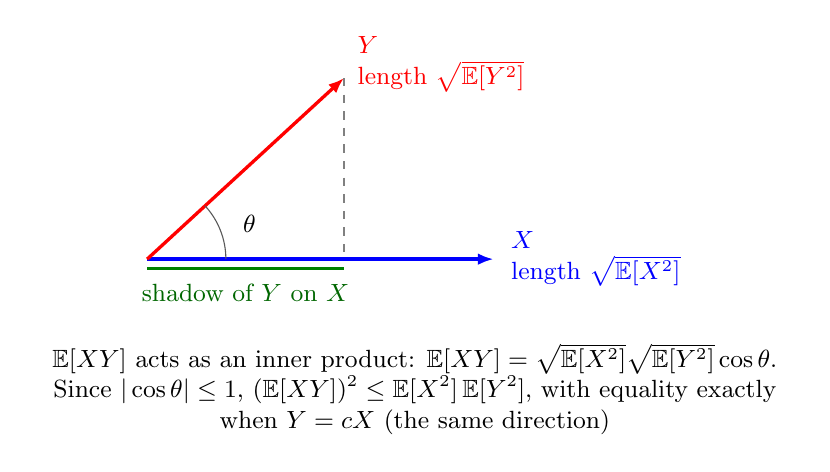
\begin{tikzpicture}[every node/.style={font=\small}, >={Latex[length=2mm]}]
	\draw[->, very thick, blue] (0,0) -- (4.4,0);
	\node[blue, anchor=west, align=left] at (4.5,0) {$X$\\ length $\sqrt{\mathbb{E}[X^2]}$};
	\draw[->, very thick, red] (0,0) -- (2.5,2.3);
	\node[red, anchor=south west, align=left] at (2.55,2.0) {$Y$\\ length $\sqrt{\mathbb{E}[Y^2]}$};
	\draw[gray, dashed] (2.5,2.3) -- (2.5,0);
	\draw[gray!70!black] (1.0,0) arc (0:42.6:1.0);
	\node[font=\small] at (1.3,0.45) {$\theta$};
	\draw[very thick, green!50!black] (0,-0.12) -- (2.5,-0.12);
	\node[green!40!black, anchor=north, font=\small] at (1.25,-0.2) {shadow of $Y$ on $X$};
	\node[anchor=north, align=flush center, text width=9.6cm] at (3.4,-0.95) {$\mathbb{E}[XY]$ acts as an inner product: $\mathbb{E}[XY]=\sqrt{\mathbb{E}[X^2]}\sqrt{\mathbb{E}[Y^2]}\cos\theta$. Since $|\cos\theta|\le1$, $(\mathbb{E}[XY])^2\le\mathbb{E}[X^2]\,\mathbb{E}[Y^2]$, with equality exactly when $Y=cX$ (the same direction)};
\end{tikzpicture}
\end{document}
